\documentclass[12pt,a4paper]{article}

\usepackage[margin=2.4cm]{geometry}
\usepackage[T1]{fontenc}
\usepackage[utf8]{inputenc}
\usepackage{graphicx}
\usepackage{booktabs}
\usepackage{array}
\usepackage{enumitem}
\usepackage{float}
\usepackage{xcolor}
\usepackage{titlesec}
\usepackage{setspace}
\usepackage{newtxtext,newtxmath}
\usepackage{caption}

\setlength{\parindent}{0pt}
\setlength{\parskip}{0.55em}
\setstretch{1.08}

\definecolor{brandblue}{HTML}{2563EB}
\definecolor{brandgreen}{HTML}{16A34A}
\definecolor{brandorange}{HTML}{F97316}
\definecolor{textgray}{HTML}{374151}

\titleformat{\section}{\normalfont\Large\bfseries\color{brandblue}}{}{0pt}{}
\titleformat{\subsection}{\normalfont\large\bfseries}{}{0pt}{}
\captionsetup{font=small, labelfont=bf}

\newcommand{\insight}[2]{%
  \textbf{#1:} #2
}

\begin{document}

\begin{titlepage}
  \centering
  \vspace*{1.4cm}

  {\Large\bfseries CENG318 - ID322\\ Human-Computer Interaction\par}
  \vspace{1.2cm}
  {\huge\bfseries Kişisel User Survey Report\par}
  \vspace{0.35cm}
  {\Large A Widget-Based Adaptive News Aggregation and Social Curation Platform\par}
  \vspace{1cm}
  {\large\bfseries Mock Survey Results and Design Implications\par}

  \vfill

  \begin{tabular}{@{}ll@{}}
    \textbf{Sample size} & N = 15 \\
    \textbf{Target group} & University-student-heavy audience \\
    \textbf{Date} & June 1, 2026 \\
    \textbf{Data source} & survey/mock\_data\_results.md \\
  \end{tabular}
\end{titlepage}

\section*{Executive Summary}

This report summarizes mock survey results collected for the Kişisel project. The goal of the survey was to validate whether users experience information overload, whether they want more control over news interfaces, and whether the project concepts of AI summaries, serendipitous discovery, editorial notes, and personal newspapers are meaningful for the target audience.

\begin{itemize}[leftmargin=1.2cm, itemsep=0.25em]
  \item \insight{Information overload is visible}{73\% of participants rated news intensity as tiring, while 93\% prefer headline or summary-level reading rather than full-context reading.}
  \item \insight{Filter bubble discomfort is strong}{80\% of participants feel that recommendation algorithms repeatedly show similar viewpoints.}
  \item \insight{Customization is highly desired}{86\% want to design their own news-reading screen and choose layout/content structure.}
  \item \insight{AI summaries fit the reading habit}{73\% would prefer short AI-generated neutral summaries for long articles.}
  \item \insight{Social curation has potential}{80\% usually add their own comment when sharing a news item, and 86\% are interested in either creating or reading a personal newspaper.}
\end{itemize}

\section*{Survey Structure}

The survey contained 12 questions grouped under four sections:

\begin{enumerate}[leftmargin=1.2cm, itemsep=0.2em]
  \item Demographics and general news habits.
  \item Problems in current news platforms, including information overload and filter bubbles.
  \item Customization, AI summarization, and serendipitous discovery.
  \item Social curation, commentary, and personal newspaper sharing.
\end{enumerate}

\section*{Participant Profile and News Habits}

\begin{figure}[H]
  \centering
  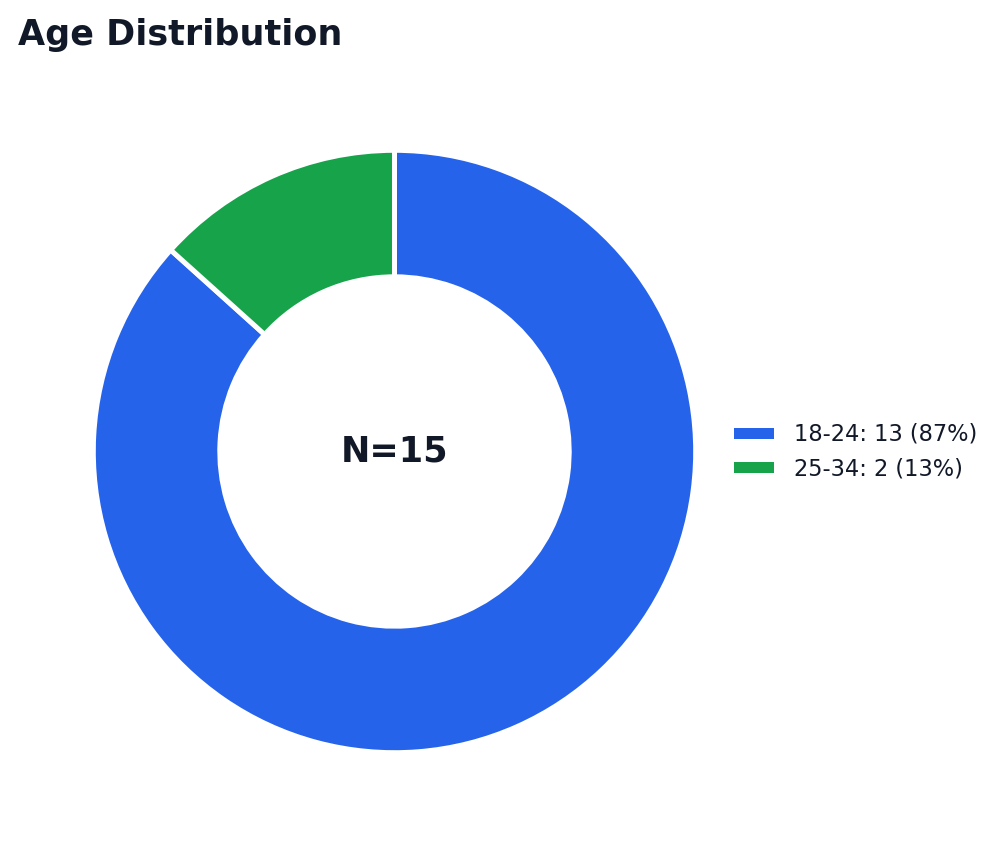
\includegraphics[width=0.72\textwidth]{figures/age_distribution.png}
  \caption{Most participants are in the 18--24 age range, matching the student-focused target audience.}
\end{figure}

\begin{figure}[H]
  \centering
  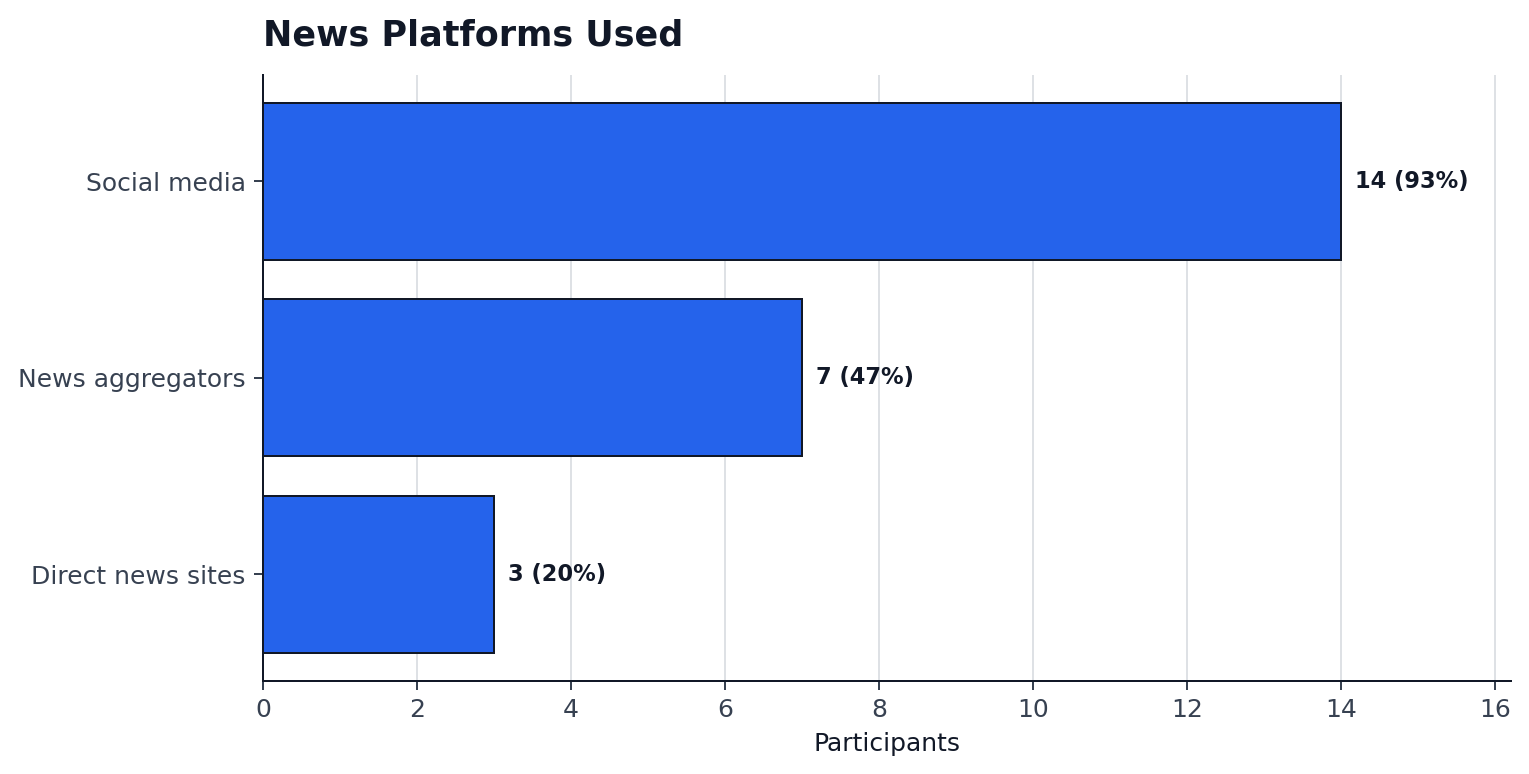
\includegraphics[width=0.88\textwidth]{figures/platforms_used.png}
  \caption{Social media is the dominant news source, followed by news aggregators and direct news sites.}
\end{figure}

\begin{figure}[H]
  \centering
  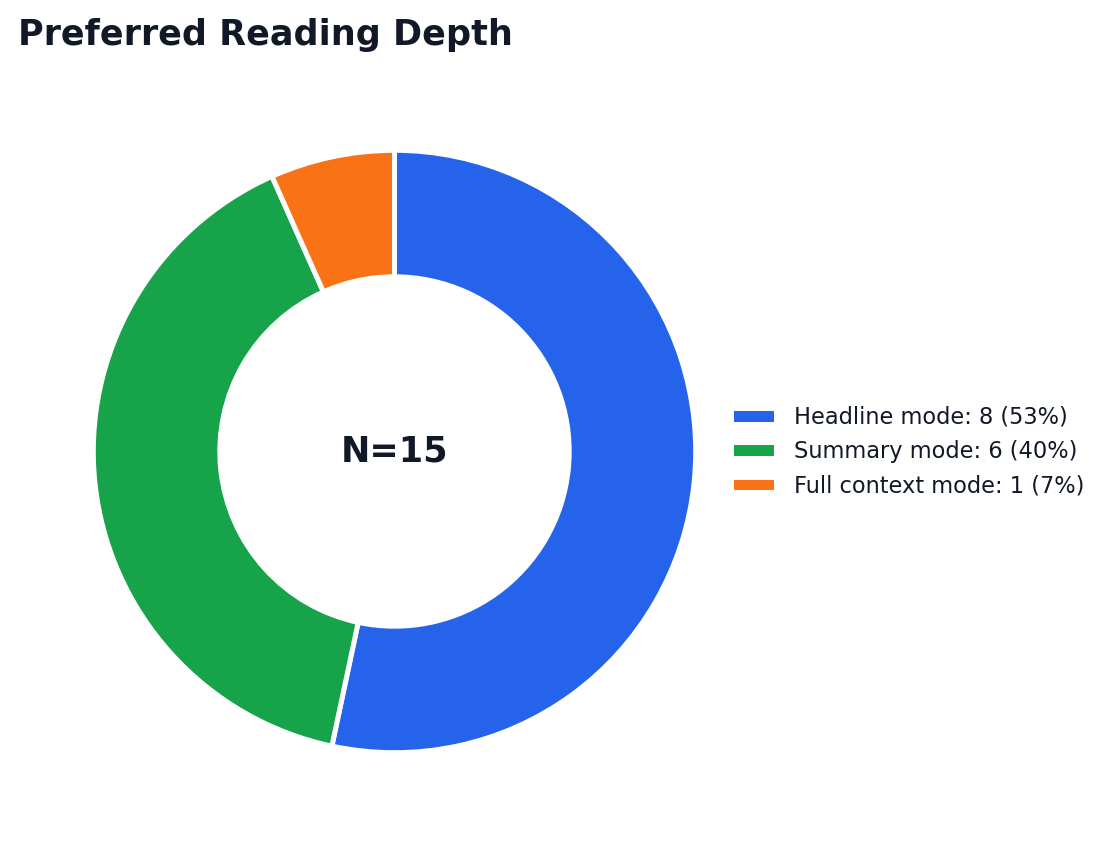
\includegraphics[width=0.76\textwidth]{figures/reading_depth.png}
  \caption{The majority of participants prefer headline or summary-level consumption.}
\end{figure}

\textbf{Design implication:} The prototype should make quick scanning efficient. The current frontend direction with Heading, Summary, and Full modes directly matches this need because only 1 out of 15 participants prefers full-context reading as the default behavior.

\section*{Problems in Current News Consumption}

\begin{figure}[H]
  \centering
  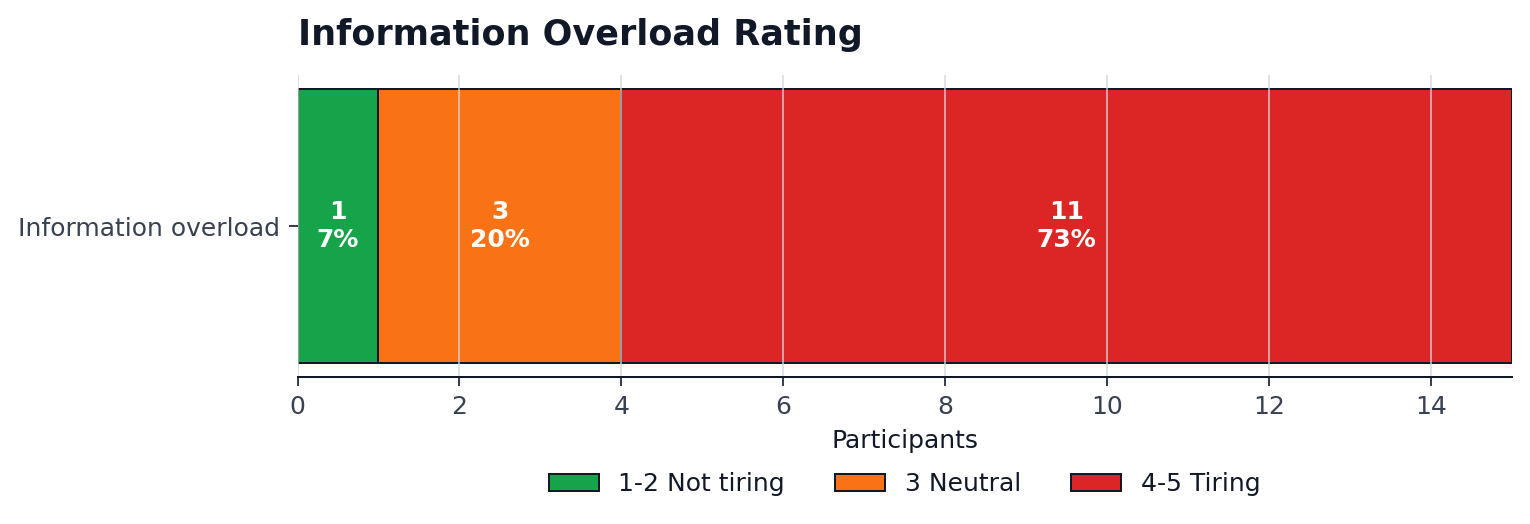
\includegraphics[width=0.9\textwidth]{figures/information_overload.png}
  \caption{11 out of 15 participants rated information overload as tiring.}
\end{figure}

\begin{figure}[H]
  \centering
  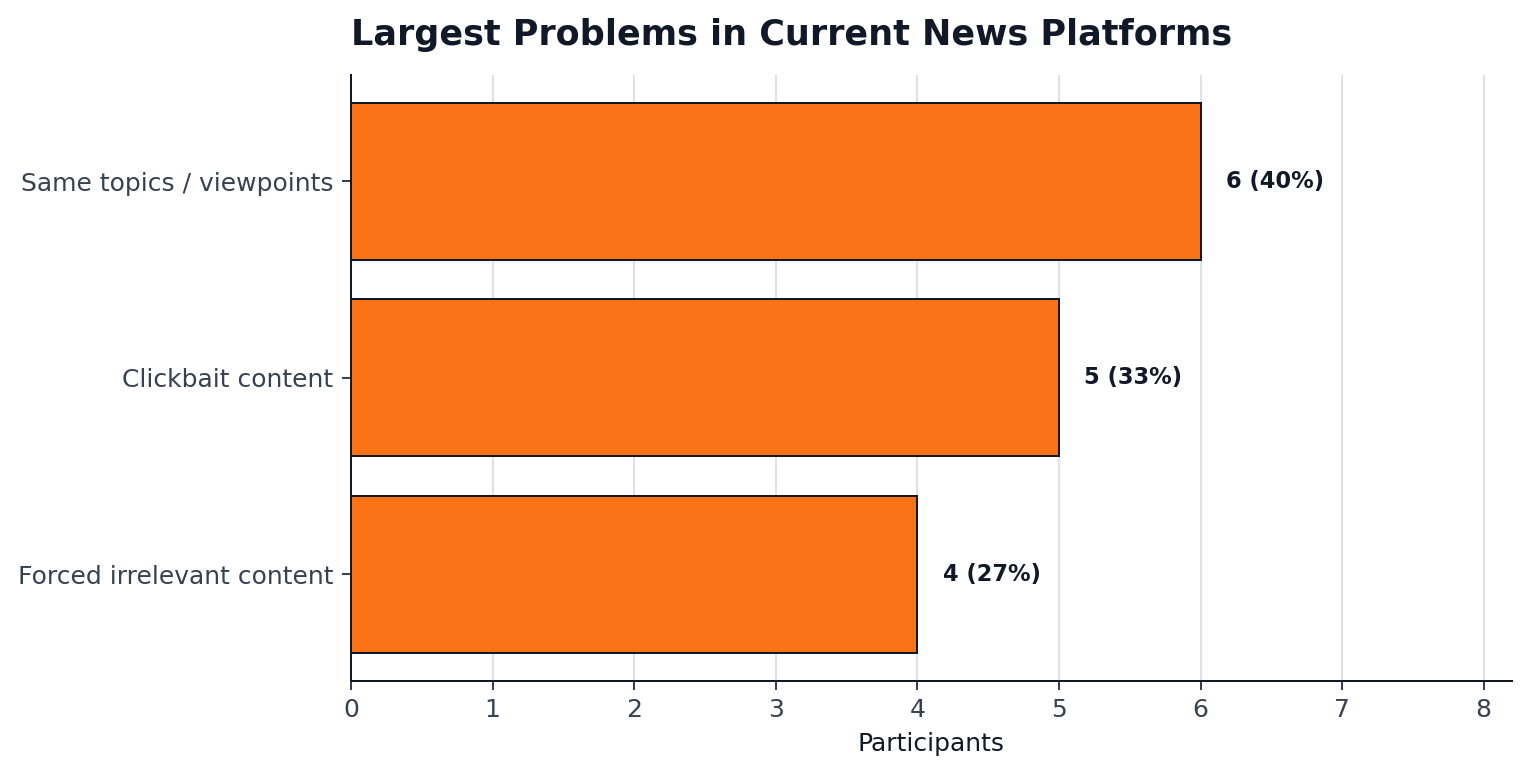
\includegraphics[width=0.9\textwidth]{figures/largest_problems.png}
  \caption{The largest reported issues are repeated viewpoints, clickbait, and irrelevant forced content.}
\end{figure}

\begin{figure}[H]
  \centering
  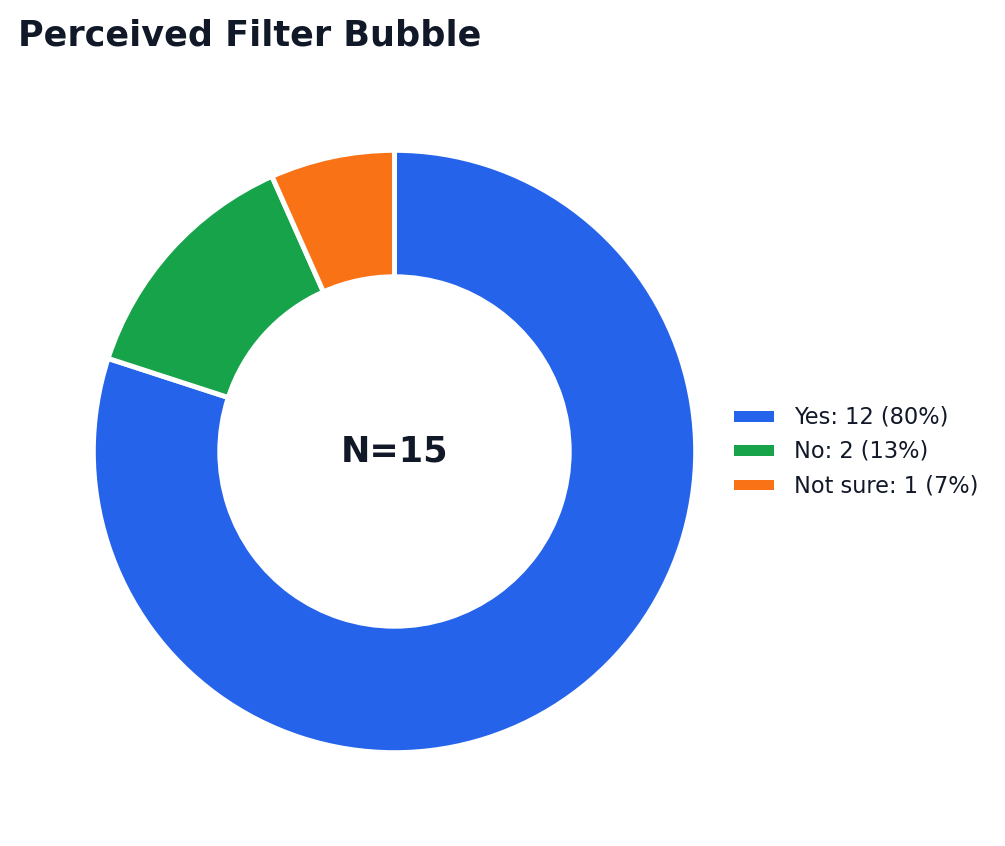
\includegraphics[width=0.76\textwidth]{figures/filter_bubble.png}
  \caption{80\% of participants feel trapped in repetitive recommendation patterns.}
\end{figure}

\textbf{Design implication:} The survey supports Kişisel's emphasis on user control and designed serendipity. Popular and Random sections should remain visible in the prototype because they respond directly to filter bubble concerns.

\section*{Validation of Proposed Features}

\begin{figure}[H]
  \centering
  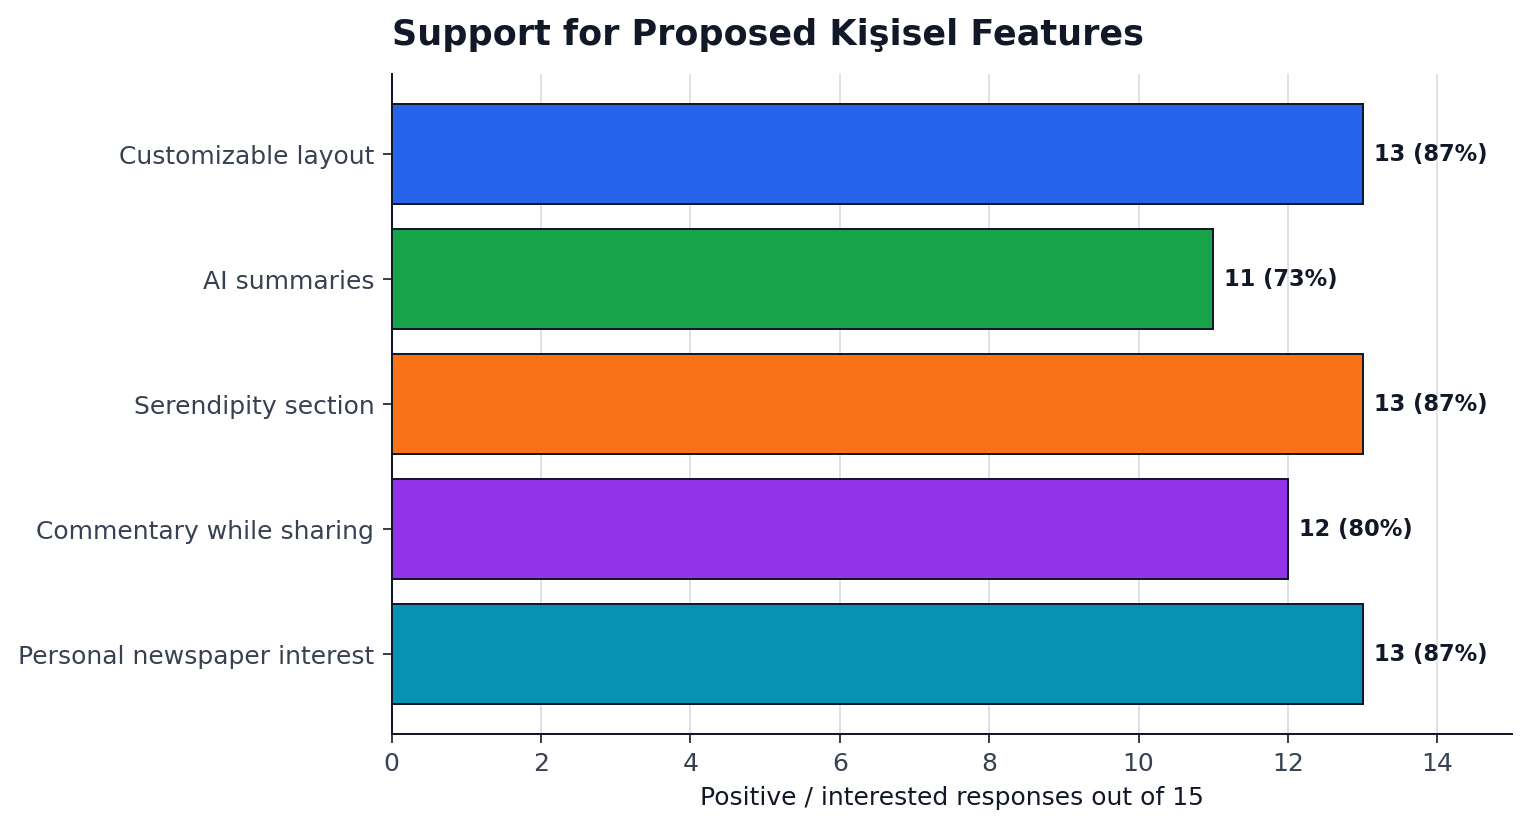
\includegraphics[width=0.92\textwidth]{figures/feature_support.png}
  \caption{Positive responses for the main proposed features of Kişisel.}
\end{figure}

\begin{table}[H]
\centering
\caption{Feature-level interpretation of survey results}
\renewcommand{\arraystretch}{1.25}
\begin{tabular}{@{}p{0.34\textwidth}p{0.18\textwidth}p{0.38\textwidth}@{}}
\toprule
\textbf{Feature} & \textbf{Support} & \textbf{Interpretation} \\
\midrule
Customizable layout & 13 / 15 & Users want control over categories, widgets, and page structure. \\
AI summaries & 11 / 15 & Short neutral summaries are a practical response to time pressure and overload. \\
Serendipity section & 13 / 15 & Random and popular news can help users escape repetitive recommendation patterns. \\
Editorial comments & 12 / 15 & Users already add comments when sharing news, so editorial widgets match an existing behavior. \\
Personal newspaper concept & 13 / 15 & Most users would either create a personal newspaper or read one curated by others. \\
\bottomrule
\end{tabular}
\end{table}

\section*{Social Curation and Personal Newspaper Concept}

\begin{figure}[H]
  \centering
  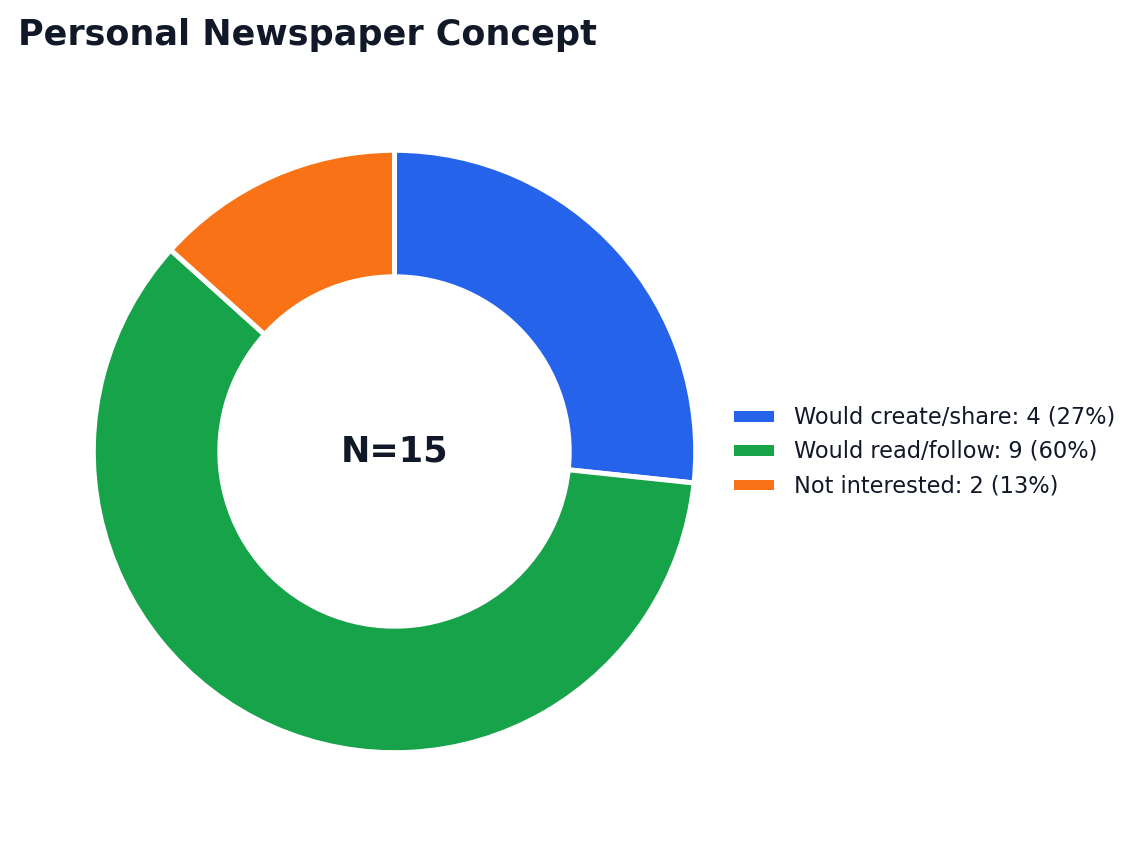
\includegraphics[width=0.76\textwidth]{figures/personal_newspaper.png}
  \caption{The personal newspaper concept has both creator and reader-side interest.}
\end{figure}

The results suggest two user roles:

\begin{itemize}[leftmargin=1.2cm, itemsep=0.25em]
  \item \textbf{Curator/commentator users:} 4 out of 15 participants would actively create and share a personal newspaper.
  \item \textbf{Reader/follower users:} 9 out of 15 participants would not necessarily create a newspaper but would read one prepared by trusted or like-minded people.
\end{itemize}

This split supports the project's social curation model. The product does not need every user to become a creator; it only needs a smaller creator group and a larger reader group for shared newspapers to be useful.

\section*{Conclusion}

The survey results support the core design direction of Kişisel. Participants report overload, repetitive recommendations, and limited agency in existing news platforms. At the same time, they show strong interest in customizable layouts, AI summaries, serendipitous discovery, editorial commentary, and shareable personal newspapers.

Based on these results, the prototype should prioritize:

\begin{enumerate}[leftmargin=1.2cm, itemsep=0.25em]
  \item A clear reading-mode control for Headline, Summary, and Full views.
  \item A customizable widget grid that gives users ownership over layout and topic selection.
  \item Editorial note controls that make commentary a first-class part of the interface.
  \item Popular and Random discovery areas to counter filter bubble effects.
  \item A simple share flow for publishing or following personal newspapers.
\end{enumerate}

\end{document}
